%!TEX program = xelatex

\documentclass[11pt,titlepage]{report}
%!TEX root = main.tex

\usepackage[T1]{fontenc}
\usepackage{lmodern}
\usepackage[svgnames]{xcolor}
\usepackage{fontspec} % XeLaTeX required!
\usepackage{graphicx}
\usepackage{circuitikz}
\usepackage{tikz}
\usepackage{pifont}
\usepackage[some]{background}
\usepackage{xltxtra} 
\usepackage{setspace}
\usepackage[absolute]{textpos}
\usepackage[latin1]{inputenc}
\usepackage[english]{babel}
\usepackage{graphicx}
\usepackage{wrapfig}
\usepackage{fullpage}
\usepackage[margin=1in]{geometry}
\usepackage{float}
\usepackage{url}
\usepackage{multicol}
\usepackage{hyperref}
\usepackage{titlepic}
\usepackage{standalone}
\usepackage{siunitx}
\usepackage{booktabs}
\usepackage{amsmath}
\usepackage{unicode-math}
\usepackage{verbatim}
\usepackage{enumitem}
\usepackage{listings}
\usepackage{multirow}
\usepackage{pgfplots}
\pgfplotsset{compat=1.8}
\usepackage{caption} 
\usepackage[parfill]{parskip}
\usepackage{import}
\usepackage[backend=bibtexu,texencoding=utf8,bibencoding=utf8,style=ieee,sortlocale=en_GB,language=auto]{biblatex}
\usepackage[strict,autostyle]{csquotes}
\usepackage[final]{pdfpages}
\usepackage{subcaption}
\usepackage{ifplatform}
%\captionsetup[table]{skip=10pt}


% Fix for includepdf bug in Mac OS X
\newcommand{\insertpdfpath}[1]{
	\ifwindows
	\newcommand{\insertpdf}[2]{\includepdf[pages=##1]{##2}}
	\else
	\newcommand{\insertpdf}[2]{\includepdf[pages=##1]{#1/##2}}
	\fi
}

%set fonts
\setmainfont[Ligatures=TeX]{Myriad Pro}
\setmathfont{Asana Math}
\setmonofont{Lucida Console}

\usepackage{titlesec, color}
\renewcommand{\familydefault}{\sfdefault} %set font family
\renewcommand{\arraystretch}{1.2} %set table vertical spacing
\setlength\parindent{0pt} %no paragraph indent
\hypersetup{ %setup hyperlinks
    colorlinks,
    citecolor=black,
    filecolor=black,
    linkcolor=black,
    urlcolor=black
}

%redesign chapter headings
\definecolor{gray75}{gray}{0.75}
\newcommand{\chapternumber}{\thechapter}
\newcommand{\hsp}{\hspace{20pt}}
\titleformat{\chapter}[hang]{\Huge\bfseries}{\chapternumber\hsp\textcolor{gray75}{|}\hsp}{0pt}{\Huge\bfseries}

%Redefine appendix headers
\renewcommand{\appendixname}{Appendix}
\renewcommand{\appendixtocname}{Appendices}
\renewcommand{\appendixpagename}{Appendices}

%For code listings
\definecolor{black}{rgb}{0,0,0}
\definecolor{browntags}{rgb}{0.65,0.1,0.1}
\definecolor{bluestrings}{rgb}{0,0,1}
\definecolor{graycomments}{rgb}{0.4,0.4,0.4}
\definecolor{redkeywords}{rgb}{1,0,0}
\definecolor{bluekeywords}{rgb}{0.13,0.13,0.8}
\definecolor{greencomments}{rgb}{0,0.5,0}
\definecolor{redstrings}{rgb}{0.9,0,0}
\definecolor{purpleidentifiers}{rgb}{0.01,0,0.01}


\lstdefinestyle{csharp}{
language=[Sharp]C,
showspaces=false,
showtabs=false,
breaklines=true,
showstringspaces=false,
breakatwhitespace=true,
escapeinside={(*@}{@*)},
columns=fullflexible,
commentstyle=\color{greencomments},
keywordstyle=\color{bluekeywords}\bfseries,
stringstyle=\color{redstrings},
identifierstyle=\color{purpleidentifiers},
basicstyle=\ttfamily\small}

\lstdefinestyle{c}{
language=C,
showspaces=false,
showtabs=false,
breaklines=true,
showstringspaces=false,
breakatwhitespace=true,
escapeinside={(*@}{@*)},
columns=fullflexible,
commentstyle=\color{greencomments},
keywordstyle=\color{bluekeywords}\bfseries,
stringstyle=\color{redstrings},
identifierstyle=\color{purpleidentifiers},
}

\lstdefinestyle{matlab}{
language=Matlab,
showspaces=false,
showtabs=false,
breaklines=true,
showstringspaces=false,
breakatwhitespace=true,
escapeinside={(*@}{@*)},
columns=fullflexible,
commentstyle=\color{greencomments},
keywordstyle=\color{bluekeywords}\bfseries,
stringstyle=\color{redstrings},
identifierstyle=\color{purpleidentifiers}
}

\lstdefinestyle{vhdl}{
language=VHDL,
showspaces=false,
showtabs=false,
breaklines=true,
showstringspaces=false,
breakatwhitespace=true,
escapeinside={(*@}{@*)},
columns=fullflexible,
commentstyle=\color{greencomments},
keywordstyle=\color{bluekeywords}\bfseries,
stringstyle=\color{redstrings},
identifierstyle=\color{purpleidentifiers}
}

\lstdefinestyle{xaml}{
language=XML,
showspaces=false,
showtabs=false,
breaklines=true,
showstringspaces=false,
breakatwhitespace=true,
escapeinside={(*@}{@*)},
columns=fullflexible,
commentstyle=\color{greencomments},
keywordstyle=\color{redkeywords},
stringstyle=\color{bluestrings},
tagstyle=\color{browntags},
morestring=[b]",
  morecomment=[s]{<?}{?>},
  morekeywords={xmlns,version,typex:AsyncRecords,x:Arguments,x:Boolean,x:Byte,x:Char,x:Class,x:ClassAttributes,x:ClassModifier,x:Code,x:ConnectionId,x:Decimal,x:Double,x:FactoryMethod,x:FieldModifier,x:Int16,x:Int32,x:Int64,x:Key,x:Members,x:Name,x:Object,x:Property,x:Shared,x:Single,x:String,x:Subclass,x:SynchronousMode,x:TimeSpan,x:TypeArguments,x:Uid,x:Uri,x:XData,Grid.Column,Grid.ColumnSpan,Click,ClipToBounds,Content,DropDownOpened,FontSize,Foreground,Header,Height,HorizontalAlignment,HorizontalContentAlignment,IsCancel,IsDefault,IsEnabled,IsSelected,Margin,MinHeight,MinWidth,Padding,SnapsToDevicePixels,Target,TextWrapping,Title,VerticalAlignment,VerticalContentAlignment,Width,WindowStartupLocation,Binding,Mode,OneWay,xmlns:x}
}

\lstdefinestyle{matlab}{
language=Matlab,
showspaces=false,
showtabs=false,
breaklines=true,
showstringspaces=false,
breakatwhitespace=true,
escapeinside={(*@}{@*)},
columns=fullflexible,
commentstyle=\color{greencomments},
keywordstyle=\color{bluekeywords}\bfseries,
stringstyle=\color{purpleidentifiers},
identifierstyle=\color{purpleidentifiers}
}

%defaults
\lstset{
basicstyle=\ttfamily\small,
extendedchars=false,
numbers=left,
numberstyle=\ttfamily\tiny,
stepnumber=1,
tabsize=4,
numbersep=5pt
}
\addbibresource{../../library/bibliography.bib}

\newcommand{\figpath}{../../deliverable-7-resources/figures}

\begin{document}

\section{Labday 5}
\subsection{Report 6}
Figure~\ref{fig:ass-2-rep-6} shows the results of our localization algorithm using the TDOA data. Note that the blue dots indicate the estimated locations using the microphone locations determined by the MDS algorithm. This algorithm is discussed in Subsection~\ref{subsec:ass-2-rep-9}. Also, the microphones are located as shown in Figure~\ref{fig:ass-2-rep-9}.

\begin{figure}[H]
	\begin{center}
		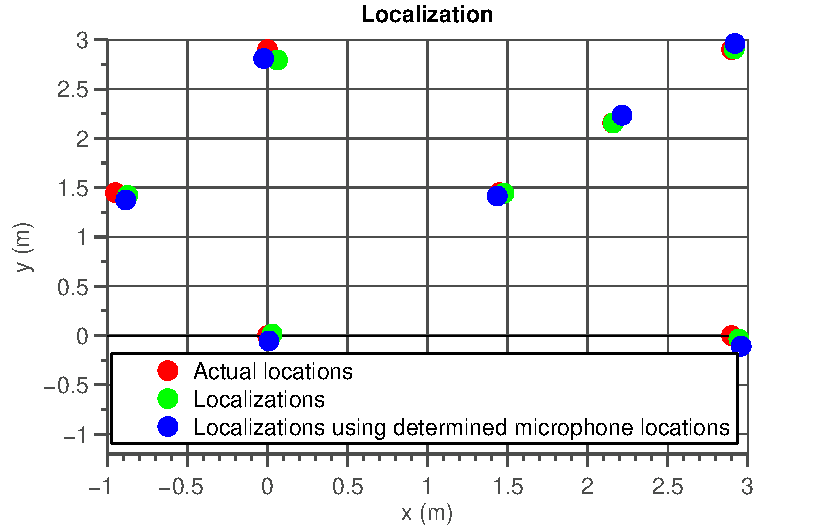
\includegraphics[width=.6\linewidth]{\figpath/ass-2/report-6/ass-2-report-6.pdf}
	\end{center}
	\caption{Localization using the TDOA data}
	\label{fig:ass-2-rep-6}
\end{figure}

The mean of the localization error is given \SI{4.92}{cm} and the STD by \SI{4.16}{cm}. If an estimated location is denoted by $\hat{\vec{x}}_i$ and the actual location by $\vec{x}$, then the error is given by $||\hat{\vec{x}}_i - \vec{x}||$. Note that the error cannot be negative. Therefore, a non-zero error average does not indicate a biased estimation.

The distance between localizations of the two points most centered is estimated \SI{0.99}{m}. The actual distance is given by \SI{1.00}{m}. This indicates good performance in de middle region.

The algorithm used is an extension of the algorithm described in the manual \cite{epo4-manual}. Thorough simulations showed that estimation is three dimensions performed worse than estimation in two dimensions. In two dimensions, the problem is overdetermined. We make use of this fact to increase the stability of our algorithm. Also, we are planning to optimize the solution by assuming that our solution is good enough to use it as a starting point for numerical optimization. Then, by fixing the third dimension -- the car does not change height -- and assuming local convexity, we should be able to improve our solution.

\subsection{Report 7}
Figure~\ref{fig:ass-2-rep-7} shows the performance of the MDS microphone localization algorithm.

\begin{figure}[H]
	\begin{subfigure}{.49\textwidth}
		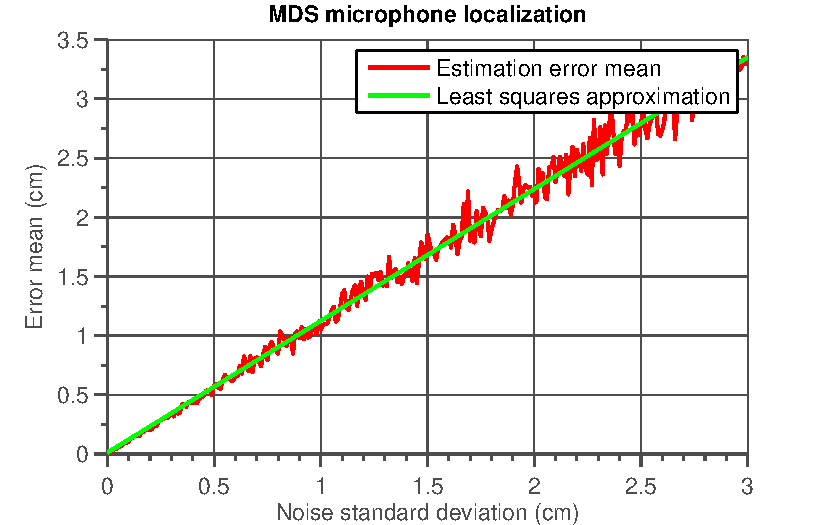
\includegraphics[width=\linewidth]{\figpath/ass-2/report-7-8/ass-2-report-7-mean.pdf}
		\caption{\centering Mean of the microphone localization error by the MDS algorithm}
	\end{subfigure}
	\begin{subfigure}{.49\textwidth}
		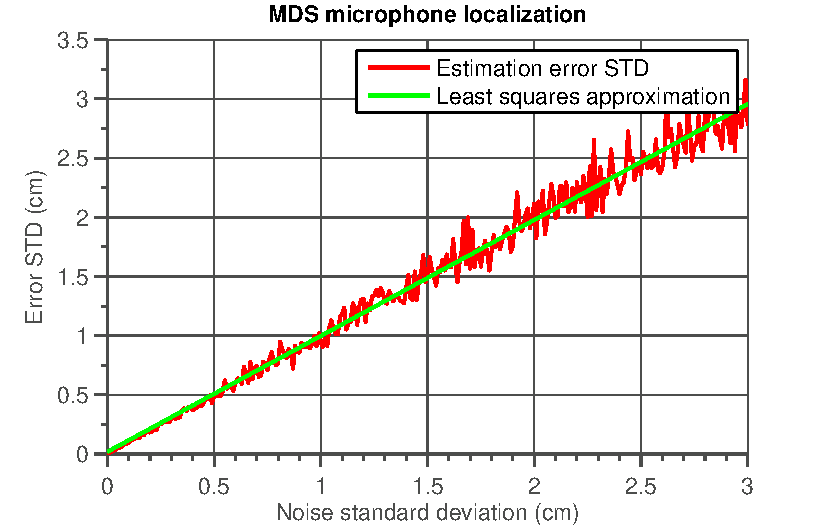
\includegraphics[width=\linewidth]{\figpath/ass-2/report-7-8/ass-2-report-7-std.pdf}
		\caption{\centering STD of the microphone localization error by the MDS algorithm}
	\end{subfigure}
	\caption{Recovered channel impulse responses through two microphones spaced various distances}
	\label{fig:ass-2-rep-7}
\end{figure}

The linear least squares approximations indicate a linear relationship between the noise standard devation and the error mean and STD. These relationships are given by
\begin{align*}
	\text{MDS localization error mean}&=1.11 \cdot \sigma_{\text{noise}}, \\
	\text{MDS localization error STD}&=0.98 \cdot \sigma_{\text{noise}}.
\end{align*}

If we eventually were to achieve a resulting $\sigma_{\text{noise}}$ of approximately \SI{3}{cm}, then this would result in an average MDS localization error and STD of also approximately \SI{3}{cm}. This is reasonable, but measuring the distances by hand would probably yield better results. We therefore expect to not rely on this algorithm.

\subsection{Report 8}
With four microphones, one is able to estimate by four measurements the distance between each pair of microphones. Their coordinates can consequently be estimated in three dimensions \cite{shang-wheeler-mds}. However, the third dimension of the car is already known. The fourth microphone could be used to improve the two dimensional estimation, which is most certainly useful.

The problem with the MDS algorithm is correcting the frame of reference. However, this problem is solved by \textbf{(1)}, defining a microphone to be at $(0,0)$ and thus introducting a point of reference, \textbf{(2)}, defining a microphone to be at $(0,+x)$ and thus introducting an angle of reference and \textbf{(3)}, defining a microphone to have a positive $y$-coordinate to create a reflectional perspective of reference. These three aspects can easily be implemented by means of elegant linear algebra.

MDS requires to have a set $\mathcal{S}$ of locations $\vec{s}_i$, $i \in \{0,1,2,\dots,n\}$ for which for each pair $\vec{s}_i$, $\vec{s}_j$, $i \neq j$, $i, j \in \{0,1,2,\dots,n\}$ the distance $||\vec{s}_i-\vec{s}_j||$ is known. If one is able to compose such a set by means of TDOA, then the relative position of each object can be found.

\subsection{Report 9}
\label{subsec:ass-2-rep-9}
Figure~\ref{fig:ass-2-rep-9} shows the results of our microphone localization using the TDOA data.

\begin{figure}[H]
	\begin{center}
		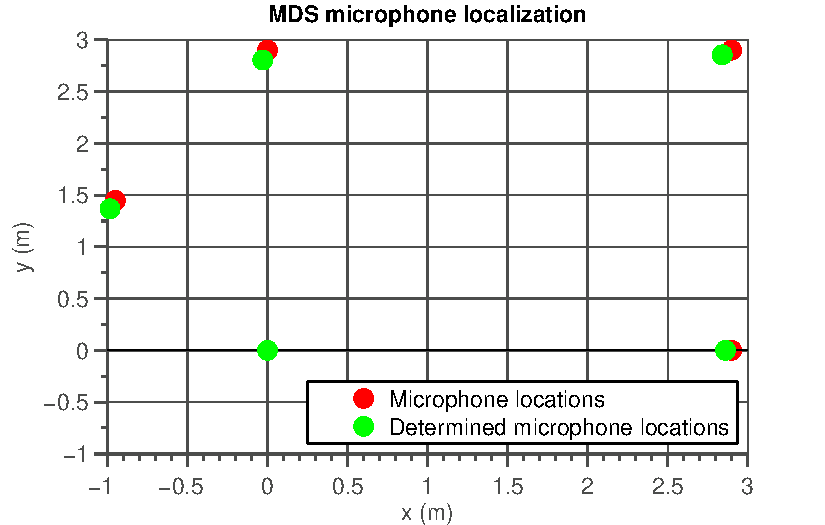
\includegraphics[width=.6\linewidth]{\figpath/ass-2/report-9/ass-2-report-9.pdf}
	\end{center}
	\caption{Microphone localization using the MDS algorithm}
	\label{fig:ass-2-rep-9}
\end{figure}

The microphone localization error average is given by \SI{6.03}{cm} and the STD by \SI{4.08}{cm}. The mentioned figure shows that the estimated microphone locations match the estimation locations pretty good. These results could probabily be used for driving KITT. However, this is by no means optimal. Further simulations showed that this method of localization is reliable if the TDOA estimation performs correctly.


	
\end{document}